%
% File acl2020.tex
%
%% Based on the style files for ACL 2020, which were
%% Based on the style files for ACL 2018, NAACL 2018/19, which were
%% Based on the style files for ACL-2015, with some improvements
%%  taken from the NAACL-2016 style
%% Based on the style files for ACL-2014, which were, in turn,
%% based on ACL-2013, ACL-2012, ACL-2011, ACL-2010, ACL-IJCNLP-2009,
%% EACL-2009, IJCNLP-2008...
%% Based on the style files for EACL 2006 by 
%%e.agirre@ehu.es or Sergi.Balari@uab.es
%% and that of ACL 08 by Joakim Nivre and Noah Smith

\documentclass[11pt,a4paper]{article}
\usepackage[hyperref]{acl2020}
\usepackage{times}
\usepackage{latexsym}
\renewcommand{\UrlFont}{\ttfamily\small}



\usepackage{amsmath}
\usepackage[linesnumbered,ruled]{algorithm2e}
\usepackage{tablefootnote}
\DeclareMathOperator*{\argmax}{arg\,max}

%\aclfinalcopy % Uncomment this line for the final submission
%\def\aclpaperid{***} %  Enter the acl Paper ID here


% This is not strictly necessary, and may be commented out,
% but it will improve the layout of the manuscript,
% and will typically save some space.
\usepackage{microtype}

%\aclfinalcopy % Uncomment this line for the final submission
%\def\aclpaperid{***} %  Enter the acl Paper ID here

%\setlength\titlebox{5cm}
% You can expand the titlebox if you need extra space
% to show all the authors. Please do not make the titlebox
% smaller than 5cm (the original size); we will check this
% in the camera-ready version and ask you to change it back.

\newcommand\BibTeX{B\textsc{ib}\TeX}

\title{A Complex KBQA System using Multiple Reasoning Paths}

\author{First Author \\
  Affiliation / Address line 1 \\
  Affiliation / Address line 2 \\
  Affiliation / Address line 3 \\
  \texttt{email@domain} \\\And
  Second Author \\
  Affiliation / Address line 1 \\
  Affiliation / Address line 2 \\
  Affiliation / Address line 3 \\
  \texttt{email@domain} \\}

\date{}

\usepackage{tikz}
\newcommand{\kechen}[1]{\textcolor{red}{[Kechen]: {#1}}}
\newcommand{\cheng}[1]{\textcolor{red}{[Cheng]: {#1}}}
\newcommand{\fix}[1]{\textcolor{blue}{[To be fixed]: {#1}}}
\newcommand{\yu}[1]{\textcolor{green}{[Yu]: {#1}}}
\newcommand{\kalpa}[1]{\textcolor{blue}{[Kalpa]: {#1}}}

\begin{document}

\maketitle

\begin{abstract}
 Multi-hop knowledge based question answering (KBQA) is a complex task for natural language understanding. Many KBQA approaches have been proposed in recent years, and most of them are trained based on labeled reasoning path. This hinders the system's performance as many correct reasoning paths are not labeled as ground truth, and thus they cannot be learned by the model. In this paper, we introduce an end-to-end KBQA system which can leverage multiple reasoning paths' information and only requires labeled answer as supervision. We conduct experiments on several benchmark datasets containing both single-hop simple questions as well as muti-hop complex questions, including WebQuestionSP (WQSP), ComplexWebQuestion-1.1 (CWQ), and PathQuestion-Large (PQL), and demonstrate strong performance.
\end{abstract}

delta-function that puts all its mass on one state

\begin{figure}[t]
 \centering
 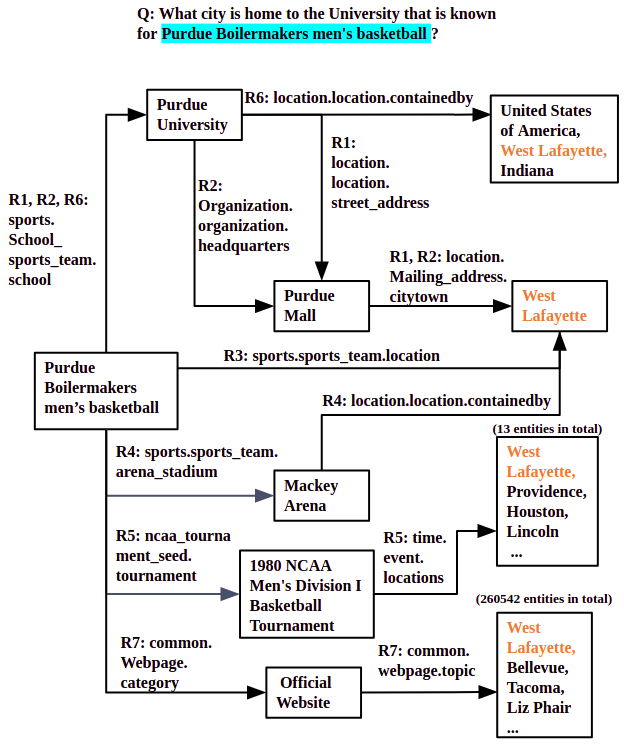
\includegraphics[width=1\linewidth]{figs/fig1.png}
 \caption{One QA example with Multiple Relation Paths from \textsc{ComplexWebQuestion}-1.1. The blue color highlighted is the extracted topic entity. Each square represents an entity, and the arrows represent the relations. Relation path $R_1$ to $R_4$ are the good ones containing meaningful relation paths to the final answer. $R_5$ and $R_6$ are the worse paths that generate a larger final answer set containing some wrong entities. $R_7$ is the worst one as its relation path is totally not interpretable and the answer set is huge.}
 \label{QAPaths}
\end{figure}

\section{Introduction}

Knowledge-based question answering (KBQA) is the task of finding answers to questions by processing a structured knowledge base $\mathcal{KB}$. %where the beliefs are stored as triples containing two entities and the relation linking them. 
A $\mathcal{KB}$ consists of a set of entities $\mathcal{E}$, a set of relations $\mathcal{R}$, and a set of literals $\mathcal{S}$. A knowledge base fact is defined as $(h,r,t)$, where $h\in \mathcal{E}$ is the head entity, $t \in \mathcal{E} \bigcup \mathcal{S}$ is the tail entity/literal, and $r\in \mathcal{R}$ is the directed relation between $h$ and $t$. To answer a simple single-relation question (\emph{i.e.} a 1-hop question) like: ``Who is the president of the United States?'', %a KBQA system first identifies the topic/focus entity (\emph{i.e.} United States) and the relation (\emph{i.e.} ``president '') asked in the question, then searches for the entity by matching the entity-relation tuple $\textless$United States, president, $?\textgreater$ over KB. \kalpa{use of a topic entity is approach specific. Many KBQA systems exist that do not use topic entity. E.g., template based QA}
a typical KBQA system first identifies the entity (\emph{i.e.} United States) and the relation (\emph{i.e.} ``president'') asked in the question, and then searches for the answer entity by matching the entity-relation tuple $\textless$United States, president, $?\textgreater$ over $\mathcal{KB}$.


While the single-hop question can be answered by searching a predicate relation in $\mathcal{KB}$, it is not trivial to answer more complex multi-hop questions containing multiple entities and relations with constraints. Take two types of multi-hop questions for example: (1) For a complex compositional question, it is not trivial to extract the correct relations in their right sequences together with the correct head and tail entities, and (2) For a complex conjunction question, it is difficult to extract multiple reasoning paths, and combine their results at the end. 

Most prior work on multi-hop KBQA focuses on improving model architecture to better fit each given question to the most optimal relation path, which is given as its ground truth, and accordingly predict the most possible reasoning path during prediction. In reality, however, it is always possible that there exists many other relation paths leading to the answer, which are not given as ground truth. %It is hard to pre-define the maximum number of hops in a complex question because different questions may need different number of hops to reach their answers.
%\kechen{list a few problems (1) it hard to control number of hops. (2) how to decompose a complex question into sub-question. (3) ...} 
%\kechen{add something to explain why the above two points lead to decomposing into two sub-tasks?}
 %with random walks \cite{DBLP:conf/emnlp/GardnerTKM13} or is formulated as a Markov decision process (MDP) based reinforcement learning problem~\cite{DBLP:conf/emnlp/XiongHW17}.
%\kechen{Most of the existing KBQA systems cannot handle these two issues simultaneously. People have to pre-define different rules to solve different type of complex querys. For example, list a few work using different pre-defined strategy to solve complex QA.}%1. use different model to train, 2. neural program
%traditional approaches consider all the paths and search for the best path among them, where their searching algorithms either leverage path-ranking algorithms with random walks \cite{DBLP:conf/emnlp/GardnerTKM13} or is formulated as a Markov decision process (MDP) based reinforcement learning problem~\cite{DBLP:conf/emnlp/XiongHW17}. Since the complexity of the searching process can grow exponentially when the number of hops increase, some recent researches add decision markers or a terminal relation to decide whether a searching path should terminate or continue, in order to reduce the searching space and complexity \cite{DBLP:conf/naacl/ChenCCNK19}.
%It is commonly observed that, by using the above mentioned algorithms, the extracted relation path may not always be the best one or even can be a wrong one. The main reason is because during training, for one question, their models are trying to learn and fit to only one possible relation path, which is given as its ground truth. \kechen{while during prediction only predict one path}In reality, however, it is always possible that there exists many other relation paths leading to the answer, which are not given as ground truth. 
As the example given in Figure \ref{QAPaths}, for the question \textit{``What city is home to the University that is known for Purdue Boilermakers men's basketball?''}, there are 7 relation paths $R_n={e^n_0\rightarrow r^n_1 \rightarrow e^n_1 \rightarrow \cdots \rightarrow e^n_{ans}}\ (n=\lbrace 1, \dots, 7 \rbrace)$%\footnote{An exchangeable way to define relation path is omitting entities in the definition, because entity is determined by given the topic entity, relations, and the knowledge base. For simplicity, we simplify this relation path definition as a list of sequential relations $(r_{1}^n, r_{2}^n, \cdots, r_{T}^n)$ in the following part of this paper.}
, leading to an answer set containing the ground truth entity ``West Lafayette'', but only R1 is labeled as the ground truth relation path in the dataset. It is unlikely for the model to infer all possible relation paths that can direct the model to the answer set containing the final answer, only based on one given training path. It is not even possible for the model to differentiate the good paths from the bad ones, which are some unreasonable paths also leading to the answer sets %containing our target answer
or some reasonable paths leading to a large predicted set which contains both correct answer and noisy results. As the example given in Figure \ref{QAPaths}, relation paths $R_1$ to $R_4$ are the good ones containing meaningful relation paths to the final answer, by executing different number of hops. Comparatively, relation paths $R_5$ and $R_6$ generate a larger final answer set containing not only the correct answer but also many other wrong entities. These paths can be treated as inferior to the top 4 paths, since they give some extra invalid answers besides the correct one. In the example, path $R_7$ is even worse as its relation path is totally not interpretable plus the final answer set is exaggeratedly large which mainly contains invalid answers, hence should not be considered as a positive relation path training sample for this question. 

%Although someone may claim that we can use multiple relation paths as ground truths for one question to improve the coverage and performance, it is still not feasible to label all valid relation paths considering the complexity of ground truth label preparation. 
%\kechen{combine this paragraph with the next paragraph? now we have two separate paragraphs to first introduce the issue and then use an example to explain it. should we combine them together?}

In this paper, we propose an end-to-end multi-hop KBQA system, which successfully leverage the training information from multiple relation paths, and learn the good relation paths over the inferior or the bad ones, by being given the labels of only one valid relation path (as in most KBQA datasets) or even no relation labels. We model the relation paths as a latent variable, and propose supporting training and prediction methods. Experimental results show that the system can output diverse relation paths, and reward the ``better'' paths over the inferior ones by assigning ``better'' paths higher probabilities. Our method can be applied to most KBQA systems to predict entity and relation, and can be used with any model architecture. We achieve state-of-the-art performance on three popular KBQA datasets for single-hop and multi-hop questions.%taking the size of their answer set into consideration, \emph{i.e.} the larger is the final answer set, the worse is a relation path, as it contains more irrelevant answer information. \kechen{modify the last sentence} %We also use a sampling approach to filter the wrong paths like $R_8$ in our example. 
% Specifically, we make the following contributions:\\
% 1. We introduce a novel multi-hop KBQA structure, which can predict the relation sequence of any length without pre-defining the number of maximum hops and generate final answers at the last hop.\\
% 2. We design a novel loss function using latent variables, such that the system can be trained without being given any ground truth relation path, or by leveraging more valid training paths information even if one ground truth path is given. We also give detailed analysis to demonstrate the benefits of using the new loss function.\\
% 3. We achieve state-of-the-art performance on three popular KBQA dataset containing single-hop and multi-hop questions.
%Specifically, we make the following contributions:
%\begin{enumerate}
%    \item We introduce a novel multi-hop KBQA system, which can leverage the information from multiple relation paths. %predict the relation sequence of any length without pre-defining the number of maximum hops and generate final answers at the last hop.
%    \item We design a novel loss function and the corresponding training and prediction methods. Detailed analysis is given to demonstrate the benefits of using this new loss function.
%    \item We achieve state-of-the-art performance on three popular KBQA datasets for single-hop and multi-hop questions.
%\end{enumerate}


\begin{figure*}[t]
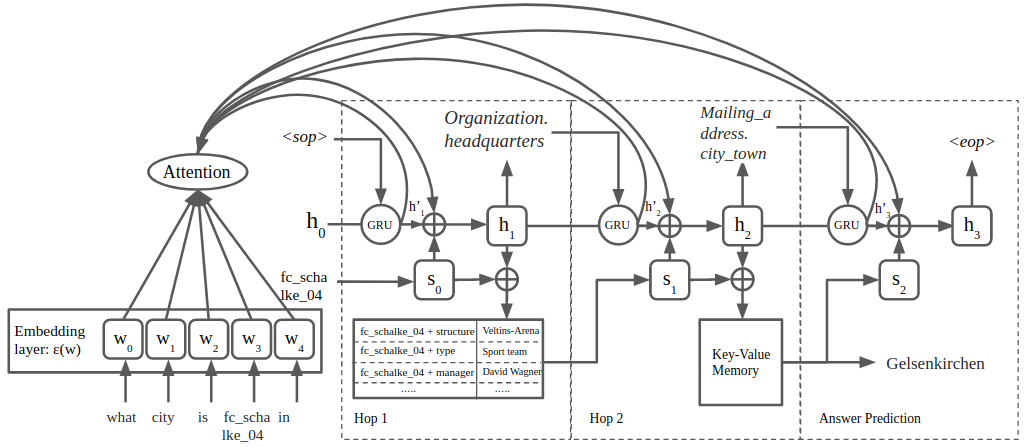
\includegraphics[width=2.1\columnwidth]{figs/model2.png}
\caption{\fontsize{10}{12}\selectfont A running example of our model to answer question \textit{What city is fc\_schalke\_04 in?}. The entity linker extracts \textit{fc\_schalke\_04} as the topic entity. $[\textit{\textless sop\textgreater}, \textit{Organization.headquarters} , \textit{Mailing\_address.city\_town, \textless eop\textgreater}]$ is the predicted relation path and \textit{Gelesenkirchen} is the predicted answer. In the diagram, we use $\bigoplus$ to represent concatenation. }
\label{fig:model}
\end{figure*}


\section{Model}
\kechen{add e to the path}
 Given a question $q$ and its topic entity $e_0$ (identified by entity linking), our model aims to find the relation path $\mathbf{r} = (r_{1}, r_{2}, \cdots, r_{T})$ and the answer $y$ from the knowledge base $\mathcal{KB}$. In this section, we first present the design of our model architecture, and then explain the training and inference algorithms in details.  

\subsection{Model Architecture}


Figure \ref{fig:model} illustrates the architecture of our model, which contains four main components as follows:

\subsubsection{Question Encoding} Given an input question $q=(w_0, w_1, \cdots, w_{|q|-1})$, we wish to learn different question context representations to show different reasoning focus at each hop. The model feeds words to an embedding layer to acquire pre-trained word embeddings $\varepsilon(w)$. 
% $\varepsilon(\cdot)$ function represents gathering embedding of the input from the corresponding pre-trained embeddings matrix. 
To reduce computational complexity, we do not use RNN to fine tune embeddings in a traditional sequence-to-sequence fashion. The output word embeddings are combined in different ways based on attention weights learned by relation prediction module at each hop.


%\subsubsection{Reasoning Decoding} The decoding module consists of relation prediction module and entity prediction module.

\subsubsection{Relation Prediction} We model relation prediction as a sequence prediction task using recurrent neural network with gated recurrent units (GRU). The hidden representations of GRU unit and predicted relation are denoted by $h$ and $r$ respectively. At timestep $t$, the model attends on particular words from the input question $q$ via attention mechanism \cite{DBLP:journals/corr/BahdanauCB14}:
\begin{align}
h'_{t} = GRU(h_{t-1}, r_{t-1}) 
\end{align}
\vspace{-3ex}
\begin{align}
u_{tk} = a(h'_{t},\varepsilon(w_k))
\end{align}
\vspace{-3ex}
\begin{align}
\alpha_{tk} = \frac{\exp (u_{tk})}{\sum_{0\leq j\leq |q|-1}\exp (u_{tj})}
\end{align}
\vspace{-1ex}
%\[\alpha_{tk} = \frac{u_{tk}}{\sum_{j}u_{tj}}\]
\begin{align}
c_t = \sum_{0\leq j\leq |q|-1}\alpha_{tj}\varepsilon(w_j)
\end{align}

where $a$ is a parameterized feed-forward neural network to calculate the similarity score of two inputs, and $c_t$ is the output of attention module as the question context vector. %After having all above computations done, 

The model then concatenates temporary hidden state $h_{t}'$, entity representation $\varepsilon(e_{t-1})$, and question context $c_t$ together, and pass the concatenation through an gating function $g(\cdot)$. This gating mechanism equips the model with ability to assign different wights on different features. At last, the model has a \textit{Softmax} output layer to generate probabilities to each candidate relation.  The process can be formally described by the following equations:
\begin{align}
[z_t^{h'}, z_t^{e}, z_t^{c}] = g([h'_{t}; \varepsilon(e_{t-1}); c_t])
\end{align}
\vspace{-2ex}
\begin{align}
h_{t} = \phi(z^{h'}_tW^{h'}h'_{t}+z^{e}_t W^{e}\varepsilon(e_{t-1})+z^{c}_t W^{c}c_{t})
\end{align}
\vspace{-2ex}
\begin{align}
o^j_t = \frac{\exp <h_t,\varepsilon(r_j)>}{\sum_k\exp <h_t,\varepsilon(r_k)>}
\label{eq:r_prob}
\end{align}

where $\phi$ represents one layer neural network with ReLU activation, $W^{(*)}$ are parameter matrices, $\varepsilon$ is the embedding gathering function, $<>$ outputs the dot product between two inputs, and $o_t^j$ is the probability of predicting the $j$-th relation in $\mathcal{R}$ at timestep $t$. After the model predicts a relation $r_t$, it can simply execute a query $(e_{t-1}, r_{t-1}, ?e_t)$ to get an entity $e_t$ from the knowledge base. The other way to collect this entity is via a soft lookup with a key-value memory network structure. We provide more details in the appendix.


\subsubsection{Objective Functions}
\kechen{add $e$ to path}
At a timestep $t$, our model take input features from three sources: question context $c$, previous entity $e$, and path history $h'$. The training objective of relation can be written using these notations as follows:


\begin{equation}
\begin{aligned}
P(r_t|q,r_1,r_2,...,r_{t-1}) = P(r_t|c_t, e_{t-1}, h'_t) \\
       = \sum_{f_t \in (c_t,e_t,h'_t)}P(z_t^f|c_t,e_{t-1},h'_t)P(r_t|f_t)
\end{aligned}
\end{equation}

Accordingly, the log probability of a sequence of relations $(r_1,...,r_{T})$ is defines as:

\begin{equation}
\begin{aligned}
P(\mathbf{r}|q) &= \prod_{t=1}^{T} P(r_t|q,r_1,r_2,...,r_{t-1}) 
\end{aligned}
\end{equation}

We also define the probability of generating an answer $y$ given a relation path $\mathbf{r}$ as:
\begin{align}
P(y|\mathbf{r},q) = 1/N
\end{align}

Finally, our training goal is to maximize the probability of generating the correct answer, and the training objective can be written as:

\begin{equation}
\begin{aligned}
\mathcal{L} &= -\log P(y|q) \\
            &= -\log(\sum_{\mathbf{r}\in \mathcal{P}}( P(y|\mathbf{r},q)P(\mathbf{r}|q))\\
            &= -\log(\sum_{\mathbf{r}\in \mathcal{P}} \sum_{t=1}^T\sum_{j=1}^{\mathcal{R}}\hat{o}^j_t{o^j_t} 1/N)
\end{aligned}
\label{obj:latent}
\end{equation}


\subsection{Training and Inference}
\kechen{merge 2.2 to 2.1.3 and create new 2.2 only for training algorithm? should we keep join objective here?}

The model can be trained in two ways: to maximize the joint probability $P(y,\mathbf{r}|q,\mathcal{KB})$, or to maximize answer probability $P(y|q,\mathcal{KB})$ directly by marginalizing out relation paths $\mathbf{r}$. The former one was adopted by many existing KBQA papers \cite{DBLP:conf/coling/ZhouHZ18}, while the later is novel to KBQA task. We now describe each objective in detail. Without loss of generality, we will omit $\mathcal{KB}$ in these formulas.



\subsubsection{Joint probability objective} This objective consists of two loss terms for prediction of relations and prediction of answer respectively. The loss on one instance is defined as follows:
\begin{align}
 \mathcal{L} = \sum_{h}\mathcal{L}_r^{h} + \mathcal{L}_e 
 \end{align}
  \vspace{-3ex}
\begin{align}
 \mathcal{L}_r^{h} = -\sum_{j=1}^{\mathcal{R}}\hat{o}^h_j\log{o^h_j},\;\;\mathcal{L}_e = -\sum_{i=1}^{\mathcal{E}}\hat{g}_i\log{g_i}
\end{align}
where $\mathcal{L}_e$ and $\mathcal{L}_r$ denote the cross entropy errors. $\hat{o}^h_j$ and $o^h_j$ represent gold distribution (one-hot representation) and predicted distribution defined by Eq. \ref{eq:r_prob} over relations at hop $h$. $\hat{g}_i$ and $g^h_i$ represent gold distribution and predicted distribution defined by Eq. \ref{eq:e_prob} over entities. Minimizing the sum of these two loss terms can be easily transformed to maximizing the joint probability of answer and the relation path:
\begin{equation}
\begin{aligned}
\mathcal{L} &= -\log P(y|\mathbf{r},q) - \log P(\mathbf{r}|q) \\
            &= -\log P(y,\mathbf{r}|q)
\end{aligned}
\end{equation}

For each QA pair, the joint objective function pushes the model to allocate all of the probability mass to the given relation path. However, this assumption does not reflect real-world reasoning procedures: Figure \ref{QAPaths} shows there could be multiple relation paths for one QA sample. 
To overcome this issue, some propose to use each relation path to construct a training instance, and the objective on one QA sample becomes \kechen{how to write prob of multiple e?}:
\begin{align}
\mathcal{L} = -\sum_{\mathbf{r}\in \mathcal{P}}\log P(y,\mathbf{r}|q)
\end{align}

where $\mathcal{P}$ is the set of relation paths of one QA sample labeled in training set. Although this objective has ability to learn from multiple relation paths, it is limited to fit the training data, which means only the labeled relation paths are considered.
 % It is not easy to enumerate all relation path with human labeling. 
 In addition, this objective has an undesired consequence in practical model training: because of the multiplication operation, the model has to assign equally high probabilities to all given relation paths in order to maximize the product of the probabilities. If only some relation paths receive high probabilities while others receive low probabilities, the production will still be low. As a consequence, the model cannot differentiate bad relation paths from good ones by assigning different probabilities to them.

\subsubsection{Marginal probability objective} We propose a new way to train KBQA model by treating relation path as latent variable, and marginalize it out to maximize the final answer probability directly:
\begin{equation}
\begin{aligned}
\mathcal{L} &=  -\log(\sum_{\mathbf{r}\in \mathcal{P}}( P(y|\mathbf{r},q)P(\mathbf{r}|q))\\
            &= -\log P(y|q)
\end{aligned}
\label{obj:latent}
\end{equation}

With our proposed training objective, in which the multiplication operation is replaced by the summation operation, it suffices to concentrate only on reasonable reasoning paths for each QA pair. Using Jensen's inequality, one can show that this marginal probability objective maximize the answer probability directly which is the learning goal of KBQA task, while joint probability objective maximizes a lower bound. Also, one can easily prove that the above objective pushes the model to assign both high or low probabilities for $P(y|\mathbf{r},q)$ and $P(\mathbf{r}|q)$. That is, a good relation path (high probability to point to the correct answer) also gets a high probability allocation. %A benefit of using our model with this objective is that the key hashing process filters out irrelevant memory slots from the full search space. During training, the smaller relation paths that point to an answer set, the larger probability mass will be assigned to this relation path. %This feature satisfies our definition of good path in the introduction. 


Training this objective requires summing up all valid relation paths from the topic entity to the answer entity in the knowledge base. Thus evaluating this objective exactly can be intractable. As we showed in the early example, some relation paths ($R_5, R_6, R_7$ in Figure \ref{QAPaths}) are not very helpful to training, and thus should be removed from training or assigned low probabilities. To achieve this goal, we first apply depth first search (DFS) algorithm with maximize 3 hops to get valid path candidates. The algorithm starts traversal from the topic entity node and ends at the answer entity node. All possible paths between the topic entity and the answer entity within 3 hops are extracted as candidates. We then set a threshold to remove paths which point to too many entities at the last hop. To further filter out bad relation paths, we propose to dynamically choose relation paths deemed as most probable by the current model during training. The overall training procedure is summarized in Algorithm \ref{alg:train}. Note that training with this algorithm does not require ground truth relation path label. Labeled relation path can be seen as plus, but not necessary. If it is given, we can either replace $\mathcal{P}$ with ground truth relation set, or train the model with joint probability objective using ground truth label first and transit to marginal probability objective after a few epochs.

\begin{algorithm}
  \SetKwInOut{Input}{Input}
  \SetKwInOut{Output}{Output}

 % \underline{function Euclid} $(a,b)$\;
  \Input{KBQA dataset $(q^{(n)},y^{(n)}, e_0^{(n)}),n=1,2,\cdots,N$, \\
  Knowledge Base $\mathcal{KB}$, \\
  Threshold $k_1$ and $k_2$. }
  \Output{Trained model parameters}
  Use DFS algorithm to get a set of paths $\mathcal{P}$ from $e_0^{(n)}$ to $y^{(n)}$.\\
  Remove paths that point to more than $k_1$ entities from $\mathcal{P}$.\\
  % Initialize model parameters\\
  \ForEach {batch}{
    % \ForEach {batch }{
      \ForEach{$(x^{n},\mathbf{y}^{n})$ in the batch}{
        Get top $k_2$ paths of $\mathcal{P}$ sorted by $P(\mathbf{r}|q)$ :\\
		  	$\{{\mathbf{r}}^n_{1},\cdots,{\mathbf{r}}^n_{k_2}, P({\mathbf{r}}^n_{1}|q^n),\cdots,P({\mathbf{r}}^n_{K}|q^n,$ $P({y}^n_{1}|{\mathbf{r}}^n_{1},q^n),\cdots,P({y}^n_{K}|{\mathbf{r}}^n_{n},q^n)\}$ \hspace{4ex}= Inference\_with\_current\_model$(q^{n},\mathcal{P}$)\\
		  	$\mathcal{P} = \{{\mathbf{r}}^n_{1},\cdots,{\mathbf{r}}^n_{k_2} \}$\\
        }  
              Update model parameters by maximizing $\sum\limits_{(q^{n},{y}^{n}) \in \text{batch}} \log \sum\limits_{\mathbf{r} \in \mathcal{P}}  P(y^{n}|\mathbf{r},q^{n}) P(\mathbf{r}|q^{n}) $
        }


    % }
  \caption{Training method for our model}
  \label{alg:train}
\end{algorithm}
\subsubsection{Inference} We adopt beam search to predict the relation path and use knowledge base lookup to predict the answer. Different from the vanilla beam search that allows to search on the full set of relations $\mathcal{R}$. We add two constraints to beam search so as to only select the valid path based on the knowledge base. (1) The first relation should get connected with the topic entity. (2) Each relation should get connected with the previous relation where uses an entity as the bridge. We then use an ensemble strategy to re-rank the searching results. Formally, given beam search outputs $\mathbf{r}_{1},\cdots,\mathbf{r}_{b}$ and $P(\mathbf{r}_{1}),\cdots,P(\mathbf{r}_{b})$, our model first use knowledge base lookup to get a list of different answer sets $\hat{y}_1,\cdots,\hat{y}_m$, where $m$ is the number of answer sets generated by $b$ relation paths, hence $m \leq b$. We then take the sum of the probabilities of relation paths $\mathbf{r}_i$ leading to the same predicted answer set and compare these sums. The final selected answer set $\hat{y}$ is the one with the maximum sum value. To represent it mathematically:
\begin{equation}
\hat{y}=\argmax_{\hat{y}_l} \sum_{i} P(\mathbf{r}_i\rightarrow \hat{y}_l)
\end{equation}
where $P(\mathbf{r}_i\rightarrow \hat{y}_l)$ is the probability of a relation path leading to the predicted answer set $\hat{y}_l$ and $l \in \lbrace 1, \cdots, m\rbrace$.
\section{Results and Analysis}

\subsection{Experimental Setup}
We conduct experiments on 3 multi-hop KBQA datasets, \textsc{PathQuestion-Large} (PQL) \cite{DBLP:conf/coling/ZhouHZ18}, \textsc{WebQuestionSP} (WQSP) \cite{DBLP:conf/acl/YihCHG15}, and \textsc{ComplexWebQuestion}-1.1 (CWQ) \cite{DBLP:journals/corr/abs-1807-09623}, and use the original train/dev/test split. For questions with multiple answers, we use each answer to construct a question-answer (QA) pair. Table \ref{tab:stats} contains statistics of these datasets. All of the three datasets use Freebase as the supporting knowledge base. For PQL, the original paper provides a subgraph of the Freebase. For WQSP and CWQ, we build a subgraph in a similar way as in \cite{DBLP:conf/emnlp/SunDZMSC18}, in order to generate the entity and relation candidates. We test three different graph embedding methods \textsc{Word2vec} \cite{DBLP:journals/corr/abs-1301-3781}, \textsc{TransE} \cite{DBLP:conf/nips/BordesUGWY13}, and \textsc{HolE} \cite{DBLP:journals/corr/TrouillonN17}, and decide to use \textsc{TransE} in our final experiment. \kechen{mention bert does not perform well here?}

\begin{table}[h]\centering
\resizebox{0.8\columnwidth}{!}{
\begin{tabular}{|l|c|c|c|c|c|}
\hline
& \#train & \#valid & \#test & max\_hops & path \textgreater 1\\
\hline
PQL2H & 1275    & 159     & 160    & 2  & -      \\
PQL3H & 1649    & 206     & 207    & 3  & -      \\
PQL+  & 2924    & 365     & 367    & 3  & -      \\
WQSP  & 2677    & 297     & 1639   & 2  & 79.4\%      \\
CWQ   & 27639        &    3519    &   3531     &   6   &    \\
\hline
\end{tabular}
}
\caption{\fontsize{10}{12}\selectfont Statistics of the datasets. %Note that CWQ dataset does not come with relation path annotation. We get max\_hops by counting the number of relations used in the SPARQL language.
}\label{tab:stats}
\end{table}

We implement our model using \textsc{tensorflow-1.4.0} and choose S-MART \cite{DBLP:journals/corr/YangC16a} and AllenNLP \cite{Gardner2017AllenNLP} as our entity linking tools\footnote{Entity linking results on \textsc{WebQuestionSP} can be found at \url{https://github.com/scottyih/STAGG}}. The best tuned parameters on development set are summarized as follows: the dynamic function for RNNs is chosen as a gated recurrent units (GRU) with 2 layers and at most 30 units in decoder. The size of the GRU unit and all other embedding layers are set as 300. The threshold $k_1$ is set to be: 15 plus the number of answers in the ground truth answer set, and $k_2$ is 2. We set the dropout rate as 0.3, and train the model using an Adam optimizer with a learning rate of $0.0005$. The Beam size is set to be 12 for both training and inference. We adopt the set accuracy, hits@1, and the average F1 score as our main evaluation metrics. %and compare our method with the following methods: 
It is worth noticing that: except our methods' results, all other experimental results are obtained from early published papers. Details of these models can be found from our referenced papers.

%We test different objective functions on WQSP and CWQ datasets. For WQSP, the dataset is originally labeled with multiple relation paths for each QA pair. We thus use them to train our model with joint probability objective. For CWQ, which does not come with any labeled relation path, we parse the given SPARQL queries into relation paths as ground truth labels in single path experiment. The multiple paths experiment is done by using both DFS and trained single path model to extract extra relation paths which points to the answer.


\subsection{Experimental Results}
\subsubsection{PathQuestion-Large} \kechen{why this is much better than the other two}
We first test our model on \textsc{PathQuestion-Large} (PQL) dataset. The original release contains two subsets: PQL2H and PQL3H, which contains only 2-hop and 3-hop questions correspondingly. In \cite{DBLP:conf/naacl/ChenCCNK19}, it then combined these two subsets and renamed the unified dataset as PQL+. The purpose is to evaluate if their model can stop at the correct number of hops or always stop at a fixed number of hops.

\begin{table}[h]\centering
\resizebox{1.01\columnwidth}{!}{%resize the table
\begin{tabular}{|l|c|c|c|}
\hline
                            & PQL2H & PQL3H & PQL+  \\
\hline
KV-MemNN \cite{DBLP:conf/emnlp/MillerFDKBW16}    & 72.2 & 67.4 & -         \\
IRN \cite{DBLP:conf/coling/ZhouHZ18}                         & 72.5 & 71.0     & 52.9     \\
HR-BiLSTM \cite{DBLP:conf/acl/YuYHSXZ17}                  & 97.5 & 87.9 & 92.9       \\
ABWIM \cite{DBLP:journals/corr/abs-1801-09893}                      & 94.3 & 89.3 & 92.6         \\
UHop \cite{DBLP:conf/naacl/ChenCCNK19}                       & 97.5 & 89.3 & 92.3      \\
\hline
Our Method-joint\_prob-nomemory         & 95.3 & 94.8 & 94.5       \\
Our Method-joint\_prob             & \textbf{98.3} & \textbf{97.1} & \textbf{97.5}         \\
\hline
\end{tabular}
}
\caption{\fontsize{10}{12}\selectfont We report set accuracy ($\%$) on PQL. For UHop, we use the best reported setup from the original paper, \emph{i.e.} ABWIM with UHop.}\label{tab:qpl}
\end{table}


The PQL dataset contains synthetic questions generated by templates, and each QA pair is labeled with only one relation path as its ground-truth. Because most of the QA pairs in PQL dataset can only find one corresponding relation path due to its very small knowledge base, we did not test our marginal probability objective on this dataset. The experiments are mainly used to show the prediction ability of our proposed base model with joint probability objective. Table \ref{tab:qpl} shows that our method's performance beats all the other approaches on all three subsets of PQL from 1$\%$ to 7.8$\%$ in terms of test accuracy. It is also worth noticing that the gap between our method to the previous state-of-the-art approach (\emph{i.e.} UHop) becomes larger when the number of hops increase from 2 to 3. This indicates that the importance of using our model, especially when the number of hops increases in questions. We also implement a baseline version of our method with only the question encoding and relation prediction modules. By removing entity lookup and answer prediction modules, our model works similarly as a vanilla RNN model with attention. The baseline model generates a sequence of relations and uses them to fetch the final answer from the knowledge base by following them sequentially. By comparing the last two rows in Table \ref{tab:qpl}, we can see that, by adding the entity lookup module, there is a significant performance boost. It equips our model with the ability not only to search but also to interact with the knowledge base. It can be further observed for Table \ref{tab:qpl} that our model performs much better than the conventional KV-MemNN, which has an entity lookup module, but does not contain a relation prediction module. We believe that this is because the intermediate key-value operations benefit from the direct relation supervision. Therefore, our model can be treated as a good combination of RNN-attention model and KV-MemNN. 
\subsubsection{WebQuestionSP}

\textsc{WebQuestionSP} is a dataset that has been widely used for relation extraction and end-to-end KBQA task. It contains 1 or 2 hops questions with ground truth relation path labels. In order to train our model with the marginal probability objective, we have two different setups by either using or not using ground truth relations to pre-train the model. Table \ref{tab:wqsp_cwq} shows that our model with marginal training objective performs much better than all other methods. KBQA-GST \cite{DBLP:conf/ijcai/LanW019} relies on additional annotations, such as textual description of the knowledge base, and using existing models to generate features. The experiments from their papers show that these generated extra features play a very important role in the system, and their F1 score drops from 67.9 to 61.5 by removing the semantic feature. Similarly, HR-BiLSTM requires relation path annotations to train their model, which are not accessible in many KBQA application scenarios. In contrast, our model supports a training method that takes only raw QA pairs as its input and does not rely on any additional labels or linguistic features. By comparing performance of using different objectives as shown in the second block of the table, we can see that there is a significant improvement by considering multiple relation paths in training. The performance gap between joint objective and marginal objective demonstrates that our proposed marginal objective is a much better way to train a model with multiple relation paths. We do not observe a very different results by using or not using labeled relation paths, which is a good signal. 


\begin{table}[h]\centering
\resizebox{1.01\columnwidth}{!}{
\begin{tabular}{|l|c|c|}
\hline
                           & WQSP & CWQ \\
\hline
KV-MemNN \cite{DBLP:conf/emnlp/MillerFDKBW16}    & 46.7 / - & 21.1\tablefootnote{The original paper only reports scores on development set.} / -      \\
HR-BiLSTM \cite{DBLP:conf/acl/YuYHSXZ17}                  & 62.9 / 62.3 & 33.3 / 31.2         \\
GRAFT-Net \cite{DBLP:conf/emnlp/SunDZMSC18}                & 67.8 / 62.5 & 30.1 / 26.0      \\
KBQA-GST \cite{DBLP:conf/ijcai/LanW019}          & 68.2 / 67.9 & 39.3 / \textbf{36.5}      \\
\hline
Our Method-joint\_prob             &    62.8 / 62.3  &   36.7 / 31.4        \\
Our Method-joint\_prob\_multiple\_paths             &  65.4 / 65.1     &    - / -       \\
Our Method-marginal\_prob\_with\_true\_label             &   \textbf{68.9} / \textbf{68.5}    &      \textbf{39.4} / 34.8     \\
Our Method-marginal\_prob\_without\_true\_label             &   68.8 / 68.3    &       33.0 / 27.6    \\
%Our Method-obj3+new\_decode  &     &          \\
\hline
\end{tabular}
}
\caption{\fontsize{10}{12}\selectfont We report hits@1 / F1 on WQSP and CWQ.}\label{tab:wqsp_cwq}
\end{table}


\begin{table*}[t]\centering
\resizebox{2.1\columnwidth}{!}{%resize the table
\begin{tabular}{l|l|l}
\hline
\multicolumn{3}{c}{Question: what state does romney live in?  \ \ \        Answer: Massachusetts  \ \ \       Topic entity: romney}                                                                                                                                            \\ \hline
.89:children & .29:education\_institution,state\_province\_region & .83:\textbf{places\_lived,location} \\ \hline
.06:\textbf{government\_positions,jurisdiction\_of\_office} & .25:\textbf{places\_lived,location} & .12:\textbf{government\_positions,jurisdiction\_of\_office} \\ \hline
.04:\textbf{government\_positions,office\_position\_or\_title} & .25:\textbf{government\_positions,district\_represented} & .04:\textbf{government\_positions,district\_represented} \\ \hline
.00:\textbf{government\_positions,district\_represented} & .01:\textbf{government\_positions,jurisdiction\_of\_office} & .01:place\_of\_birth,state \\ \hline
.0:place\_of\_birth & .01:place\_of\_birth,state & .00:education,degree \\ \hline
.00:jurisdiction\_of\_office & .01:sibling,place\_of\_birth & .00:election\_campaigns \\ \hline 
\multicolumn{3}{c}{Question:where did madonna grew up?\ \ \       Answer: Bay City\ \ \    Topic entity: madonna}                                                                                                                                            \\ 
\hline
.99:\textbf{place\_of\_birth} & .50:nominated\_for & .47:nominated\_for,featured\_film\_locations \\ \hline
.00:nominated\_for & .16:nominated\_for,featured\_film\_locations & .40:\textbf{place\_of\_birth} \\ \hline
.00:\textbf{place\_lived.location} & .11:compositions & .11:\textbf{place\_lived.location,place} \\ \hline
.00:place\_lived.location,containedby & .09:\textbf{place\_lived.location} & .00:nominated\_for \\ \hline
.00:compositions & .08:\textbf{place\_of\_birth} & .00:\textbf{place\_lived.location} \\ \hline
.00:religion & .01:award\_nominations,nominated\_for & .00:\textbf{place\_lived.location,region} \\ \hline


\end{tabular}
}\caption{\fontsize{10}{12}\selectfont Two running examples from \textsc{WebQuestionSP} dataset. We show the probability $P(\mathbf{r}|q)$ before the inferred relation path. Relation paths that lead to the correct answers are highlighted in bold. The three columns are corresponding to the results by using joint objective with single path, joint objective with multiple paths, and marginal objective with multiple paths. Due to space limit, we only show the partial name of a relation in the example and the probability less than .01 is shown as .00.}\label{tab:case}
\end{table*}

\subsubsection{ComplexWebQuestion-1.1}

This dataset is designed to study complex questions by adding more constraints to questions in \textsc{WebQuestionSP}. It contains more difficult questions than the first two datasets.  We report the experimental results in Table \ref{tab:wqsp_cwq}. Note that this dataset does not come with multiple relation path labels, so the corresponding experiment is not available. Our model outperforms all other models in terms of hits@1, and slightly worse than KBQA-GST in terms of F1 score, but again, KBQA-GST requires many additional information to train. Different from the observation in \textsc{WebQuestionSP} dataset, we see that there is a performance degradation when the model is not pre-trained with ground truth relations. It is because that the model can easily make errors in early stage and gets stuck with these errors. In contrast, our model on WQSP does not suffer from this problem because the relation path is much shorter, and thus it is not hard to generate correct training samples at the beginning of the training. To compare it with existing methods, our model still performs better than GRAFT-Net, which is the state-of-the-art results without using any additional labels.
%\section{Objective Analysis}

 %For each QA pair, the joint objective function pushes the model to allocate all of the probability mass to the given reasoning path. However, this assumption does not reflect real-world reasoning procedures. Figure \ref{QAPaths} shows there could be multiple reasoning paths for one QA sample. \cheng{list issues...cheng!} 
 
 %Although this objective has ability to learn from multiple reasoning paths, it is limited to fit the training data, which means only the labeled reasoning paths are considered. It is not easy to enumerate all reasoning path with human labeling. In addition, this objective has an undesired consequence in practical model training: because of the multiplication operation, the model has to assign equally high probabilities to all given reasoning paths in order to maximize the product of the probabilities. If only some reasoning paths receive high probabilities while others receive low probabilities, the production will still be low. As a consequence, the model cannot differentiate bad reasoning paths from good ones by assigning different probabilities to them. \cheng{list issues...cheng!} 

%\kechen{rephrase} One can easily prove that the above objective pushes the model to assign both high or low probabilities for $P(y|\mathbf{r},q)$ and $P(\mathbf{r}|q)$. It means that good relations always get high probabilities. A benefit of using our model with this objective is that key hashing process filter out irrelevant memory slots from the full search space. During training, the smaller relation paths that point to an answer set, the larger probability mass will be assigned to this relation path. This feature satifies our definition of good path in the introduction. 

%With our proposed training objective, in which the multiplication operation is replaced by the summation operation, it suffices to concentrate only on reasonable reasoning paths for each QA pair. Also, using Jensen's inequality, one can show that this marginal probability objective maximize the answer probability directly which is the learning goal of KBQA task, while joint probability objective maximize a lower bound on the log likelihood.   \cheng{list issues...cheng!} 



\section{Case Study}\label{sec:case}

%\subsection{Threshold Analysis}

Our model requires inference while using the current model to select training samples for next batch in training (see line 6 in Algorithm \ref{alg:train}). This EM style training approach helps us filter out bad relation paths based on context information. For example, a sample question from WQSP is \textit{who was the owner of kfc?}, the graph search algorithm can easily extract two ``correct'' paths starting from the topic entity \textit{kfc} directing to the ground truth answer \textit{Colonel Sanders}: \textit{kfc $\rightarrow$ organization.organization.founders $\rightarrow$ Colonel Sanders} and \textit{kfc $\rightarrow$ advertisingcharacters.product.advertising\_characters $\rightarrow$ Colonel Sanders}. However, the second path is totally wrong given that the relation path is irrelevant to the given question. \textit{Colonel Sanders} happens to be the advertising character of \textit{kfc}, but this cannot be generalized to other cases. Without using the trained model to filter out this irreverent path, the model may learn incorrect map from \textit{who is the owner...} to the relation \textit{advertising\_characters}. In our experiment, we observe that when we train our model with all relation paths generated from DFS algorithm without using this filtering strategy (\emph{i.e.} $k_2=inf$), the F1 score drops $3.4\%$ as shown in Table \ref{tab:wqsp_cwq_ablation}.

Next we demonstrate the benefit of maximizing conditional mutual information instead of likelihood. A sample question in WQSP is \textit{who did benjamin franklin get married to?}. We observe that there are 13 questions are using \textit{Benjamin Franklin} as the topic entity in the training set, but most of them are related to his invention and none of them is about marriage. With such a strong prior on \textit{Benjamin Franklin}, our experimental result shows that the model trained with maximum likelihood maps this question to a path related to \textit{invention}, while the model trained with mutual information make the correct prediction. Table \ref{tab:wqsp_cwq_ablation} shows that we get $1.8\%$ performance boost by using mutual information.




%\subsection{Case Analysis}

We further show how output probabilities look like with different training settings in Table \ref{tab:case}. In the given example, only our method outputs the correct path, and one can also find that the top three results correspond to three different but correct reasoning processes. We observe that in the training data many questions containing phrase \textit{``live in''} contains the topic entity as ``children", which explains why the first model makes wrong prediction. %In the second example, the top one ranked path of our model is not correct. However, with marginalizing out  strategy, it re-discover the correct answer by considering cumulative probabilities of it.
We can see that training with joint objective given a single relation path generates the most sharp relation path distribution, \emph{i.e.} the gap between the top entity and the second one is larger than that using other objectives. It basically only assigns probability to the top relation path. In this case, the model does not have ability to identify multiple relation paths during inference. The other extreme is that the second model is trained with joint objective and multiple input paths, which distribute probabilities over many relation paths, hence the model cannot distinguish good relation paths from the bad ones. Between the above two extremes is the proposed marginal objective with multiple input paths, when the most probable path is assigned with the largest probability, while the rest ones still get reasonable probability assignments. %In this case, it is possible to apply ensemble prediction method to combine the results of beam search outputs and re-rank them. %In our experiment, we observe 1\% performance boost on WQSP in terms of F1 using ensemble prediction method instead of simply selecting the top searching result of beam search as the prediction.

%Another interesting observation is that given the probability of the predicted relation, our model can judge the correctness of the predictions. By filtering out the test samples where the model do not show confidence (\emph{i.e.} probability of the top relation path is less than 0.9), we observe significant improvements on all three models. For example, the F1 score of the third model improves from 0.685 to 0.774 after removing 489 samples on WQSP. It shows the potential to use a second model to further re-rank our prediction results.


%\subsection{Knowledge based Question Answering (KB-QA)}
\section{Related Work}
%Most of the early KB-QA models are designed for QA problems that can be answered by a single hop, where one hop is defined as the traversal from one entity to another via a single relation. 

Most of the existing multi-hop KBQA systems %\cite{DBLP:conf/acl/YuYHSXZ17,DBLP:journals/corr/abs-1801-09893,DBLP:conf/coling/ZhouHZ18,DBLP:conf/naacl/ChenCCNK19} 
approach this task by decomposing it into two sub-tasks:
%Currently, there are mainly two main categories of methods to tackle the complex KBQA problems, the first category is based on semantic parsing, and the other category mainly relies on the embeddings (XXX) for information retrieval (IR). %Their differences will be discussed further in the relation work section, and i
%In this paper, we focus on the second category, \emph{i.e.} the embedding based approach, which can either predict the answer directly (XXX) or search (a) relation path(s) leading to the final answer entity (XXX). Conventionally, the relation path searching algorithm consists two main subtasks
topic/focus--entity linking and relation extraction. The topic--entity linking gives the system an entry point to start searching, and the relation extraction is used to search relation paths leading to the final answer. %Unlike the simple single relation questions, for complex questions, the path to the final answer may contains multiple hops, where one hop is defined as a searching step between one entity to another via a single relation. 
%For entity linking, there exists many off-the-shell tools  \cite{DBLP:journals/corr/YangC16a} that can give decent performance, and most of the current KBQA models rely on them. For relation extraction, traditional approaches consider all the paths as candidates and search for the best one among them using ranking algorithms. 
%Following this track, existing multi-hop KBQA approaches can be categorized into three groups. 
Following this track, a straightforward idea is to match the question to a candidate entity/relation directly via calculating the similarity between them \cite{DBLP:journals/corr/abs-1801-09893,DBLP:conf/adbis/YuHYZW18,DBLP:conf/ijcai/LanW019}. This method is not very suitable for multi-hop questions with long paths, because the number of candidate entity-relation combinations grows exponentially as the number of hops increases. To tackle this issue, people propose to decompose the input question into several single-hop questions, and use the existing method to solve each simple question. The decomposition methods are based on semantic parsing \cite{DBLP:conf/www/AbujabalYRW17,DBLP:conf/emnlp/LuoLLZ18} or templates \cite{DBLP:journals/corr/abs-1908-11053}. A similar idea is to encode the reasoning information hop by hop, and predict the final answer at the last hop \cite{DBLP:conf/emnlp/MillerFDKBW16,DBLP:conf/coling/ZhouHZ18,DBLP:conf/naacl/ChenCCNK19}, which is a group of methods that are more capable of handling multi-hop questions. 
%\newcite{DBLP:conf/acl/LiYSLYCZL19} casts the task as a multi-turn question answering problem, where the extraction of entities and relations is transformed to the task of identifying answers of template questions. 
It is also popular to enhance ERL results by using multi-task learning with the help of additional annotations \cite{DBLP:conf/aaai/DengXLYDFLS19,DBLP:conf/ijcai/ShaoGBJCLD19}. 

Another line of work has looked at solving KBQA task with only final answer as supervision. \newcite{DBLP:conf/acl/LiangBLFL17} first propose to model KBQA as a program generation task using neural program induction (NPI) techniques. They learn to translate the query to a program like logical form executable on the KB. As a follow up, \newcite{DBLP:conf/ijcai/AnsariSKBSC19} improves this idea by incorporating high level program structures. Both these NPI models do not require annotated relation path as supervision, but they need some prior knowledge to design the program templates. In other work, \newcite{DBLP:journals/corr/abs-1909-04849} recently propose a latent variable approach which is similar to the one described here, but applied on text-based QA scenarios. The main difference between our work is that our method aims at finding multiple reasoning paths directing to the answer, while their method only focuses on extracting one optimal solution. We employ inference during training to filter our irrelevant paths, while they use it to identify the optimal solution as training target.

\section{Conclusion}

In this paper, We introduce a novel KBQA system which can leverage information from multiple reasoning paths. The system can output diverse relation paths, and reward the ``better'' paths over the inferior ones by assigning ``better'' paths higher probabilities. To train our model, we propose to use a marginalized probability objective function and give detailed analysis to demonstrate the benefits of using the it. Experimental results show that our model achieve strong performance on three popular KBQA datasets.


\clearpage
\newpage

\bibliography{ref}
\bibliographystyle{acl_natbib}
\end{document}
